\documentclass[a4paper,10pt,hidelinks]{scrartcl}

% packages
\usepackage[ngerman]{babel}
\usepackage{graphicx}
\usepackage{hyperref}
\usepackage{url}
\usepackage{fontspec}
    \setmainfont{Arial}
    \setsansfont{Arial}
    \setmonofont{Fira Code}
\usepackage{fancyhdr}
\usepackage[paper=a4paper,left=20mm,right=20mm,top=40mm,bottom=25mm,headheight=40mm]{geometry}
\usepackage{tabto}
\usepackage{sectsty}
\usepackage{afterpage}
\usepackage{listings}
\usepackage{blindtext}
\usepackage{titlesec}

% global options
\renewcommand{\baselinestretch}{1.25}

\lstset{basicstyle=\small\ttfamily,captionpos=b,xleftmargin=0.25in,xrightmargin=0.25in}

% header/footer
\pagestyle{fancy}
\renewcommand{\headrulewidth}{0pt}
\renewcommand{\footrulewidth}{0pt}
\rhead{
\includegraphics[width=40mm]{pics/header-2.png}}
\rfoot{
\includegraphics[width=40mm]{pics/footer.png}}
\fancypagestyle{firstpage}{
    \rhead{
\includegraphics[width=40mm]{pics/header-1.png}}
}
\cfoot{}

\newcommand{\imgref}[1]{{Abbildung \ref{#1}, Seite \pageref{#1}}}

\begin{document}

\section*{\fontsize{18}{20}\selectfont Object detection in fine-art photography}
\thispagestyle{firstpage}

\textbf{Themenbereiche:} \tabto{4cm} Artificial Intelligence, Visual Computing

\noindent
\textbf{Studierender:} \tabto{4cm} Fabian Meyer

\noindent
\textbf{Betreuungsperson:} \tabto{4cm} Dr. Simone Lionetti

\noindent
\textbf{Experte:} \tabto{4cm} Roman Bachmann, Swisscom

\noindent
\textbf{Keywords:} \tabto{4cm} Object detection, Machine learning, Computer vision, Photography

\section{\fontsize{14}{16}\selectfont Aufgabenstellung}

Object detection is an important computer vision and machine learning task that consists in the localisation and classification of items within digital images. The business and industry applications of this technology are growing in number and relevance, especially because of the tremendous progress, largely driven by deep learning, that has been made in recent years.

The success of object detection models is usually measured with benchmark metrics on standard datasets such as MNIST, PASCAL VOC, ImageNet, COCO and Open Images. These reference scores summarise a complex set of performance parameters and are essential for a meaningful comparison of different approaches. Precisely because they are extremely synthetic, however, it is important to assess the quality of results with other, more ingenuous criteria.

\section{\fontsize{14}{16}\selectfont Ergebnisse}

The following results have been made:

\begin{itemize}
	\item A dataset from different artists with different styles has been gathered
	\item Multiple object detection models have been tested on images of fine-art photography
	\item The most promising model (Mask R-CNN) has been selected
	\item An program that takes in an image and puts out a tidied up version with all objects found has been developed
	\item The program has been converted into a webapp
	\item ...
\end{itemize}

\noindent
The webapplication can be viewed at: \url{http://bdaf20-iameyer.enterpriselab.ch}.

\noindent
Performance of the Mask R-CNN model depends on:

\begin{itemize}
	\item Class of objects in the image (included in COCO-dataset or not)
	\item Size of objects in the image
	\item Degree to which an object is visible and is shown in a natural style
\end{itemize}

\noindent
When applied to images of fine-art photography we can observe that performance is very variable because different photographers use a different style to depict their objects in their images. For example when using an image with a lot of small objects, performance is poor compared to an image with less number and bigger objects.

\section{\fontsize{14}{16}\selectfont Lösungskonzept}

The webapplication takes in images either from a selection or via upload or via a url. Then the model starts inference on the chosen image. The chosen model will detect potential objects in the image and returns them as masks, bounding boxes, name of class and a confidence score. \newline The program takes in the four results from the model and cuts out all objects from the original image. The found objects will be depicted on a new image in a grid-like fashion.

Cutting out the objects is possible with the bounding box and the object mask. One can cut out an object with the bounding box and colour all pixels for example white which do not belong to the mask.

\begin{figure}
    \centering
    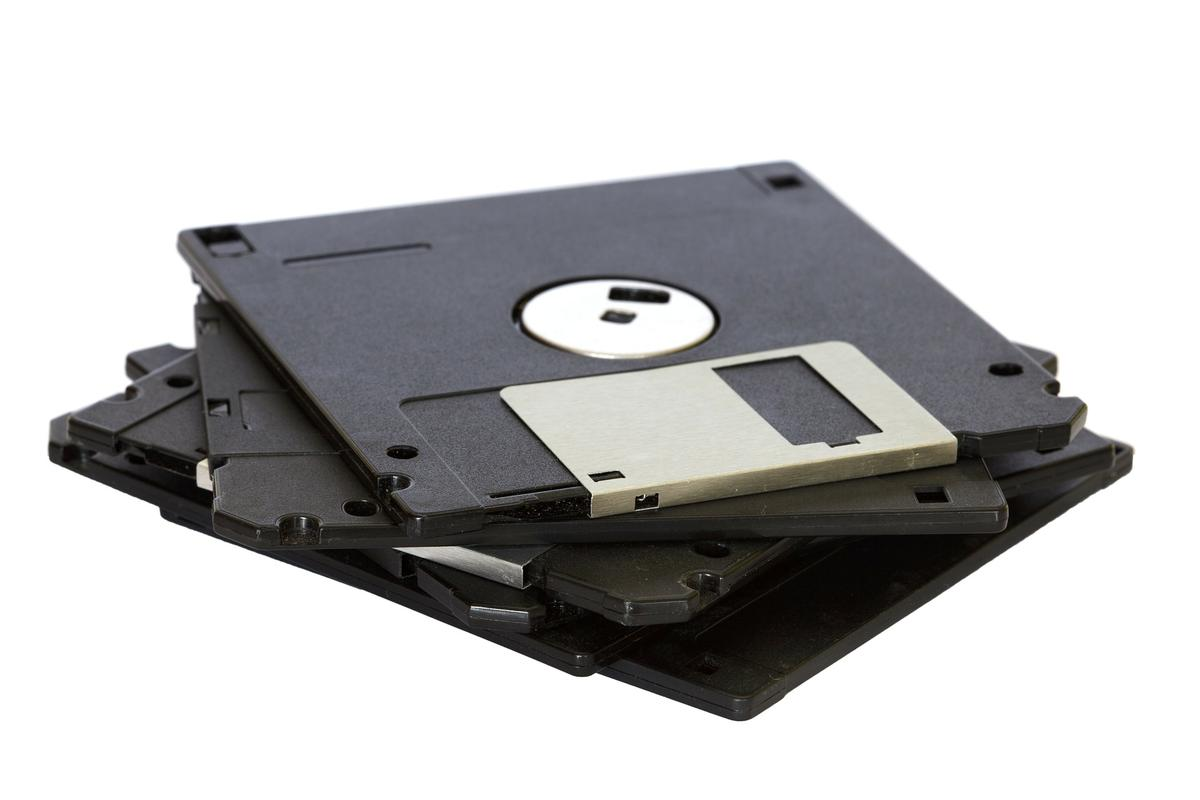
\includegraphics[width=0.4\linewidth]{pics/storage-new.jpg}
    \caption{Die Storage-Lösung für das nächste Jahrtausend}
    \label{fig:storage-new}
\end{figure}

Die erneuerte Storage-Lösung des Enterprise Labs ist in \imgref{fig:storage-new} dargestellt.

\section{\fontsize{14}{16}\selectfont Spezielle Herausforderungen}

The biggest challenge was to get a model run on a standard CPU, for development but also for deployment on a server. As most deep learning networks are trained with GPUs, the easiest way to deploy an app would be to use a GPU environment. But there are some frameworks that can accept GPU-trained networks and can use CPU for inference.

\section{\fontsize{14}{16}\selectfont Ausblick}

Die bestehende Storage-Lösung des Enterprise Labs ist in \imgref{fig:storage-old} dargestellt.

\begin{figure}
    \centering
    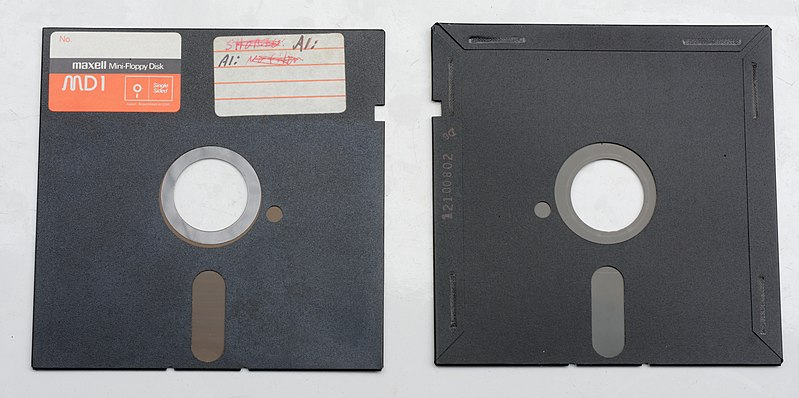
\includegraphics[width=0.5\linewidth]{pics/storage-old.jpg}
    \caption{Die bestehende Storage-Lösung im Enterprise Lab}
    \label{fig:storage-old}
\end{figure}

\end{document}
